\documentclass[abstract=off,10pt,a4paper,bibliography=totocnumbered]{article}
\usepackage[paper=a4paper,left=35mm,right=35mm,top=25mm,bottom=30mm]{geometry}
\usepackage[doublespacing]{setspace}
\usepackage[english]{babel}
\usepackage[utf8]{inputenc}
\usepackage[round]{natbib}
\usepackage{amsmath}
\usepackage{colortbl}
\usepackage{amsfonts}
\usepackage{amssymb}
\usepackage{gensymb}
\usepackage{graphicx}
\usepackage{tikz}
\usepackage{enumerate}
\usepackage{enumitem}
\usepackage{subcaption}
\usepackage{booktabs}
\usepackage[hidelinks]{hyperref}
\usepackage[nameinlink]{cleveref}
% \usepackage{lineno}
\usepackage{multirow}
\usepackage{arydshln}
% \usepackage[nomarkers, nolists]{endfloat}
\usepackage[flushleft]{threeparttable}
\usepackage{pdflscape}

%------------------------------------------------------------------------------
%	Some Styling
%------------------------------------------------------------------------------
% Creating some TikZ styles
\tikzset{
  nonterminal/.style = {rectangle
    , minimum size = 6mm
    , very thick
    , draw = black!
  }
}

% Changing the style of captions in figures etc.
\captionsetup{labelfont=bf, format=plain, font=small}

% For supplementary material
\newcommand{\beginappendix}{%
  \setcounter{table}{0}
  \renewcommand{\thetable}{S\arabic{table}}%
  \setcounter{figure}{0}
  \renewcommand{\thefigure}{S\arabic{figure}}%
  \setcounter{equation}{0}
  \renewcommand{\theequation}{Equation S\arabic{equation}}%
  \setcounter{section}{0}
  \renewcommand{\thesection}{A.\arabic{section}}%
}

%------------------------------------------------------------------------------
%	Titlepage: Header
%------------------------------------------------------------------------------
\title{\textbf{Appendix}\\ A Thee-Step Approach for Assessing Landscape
Connectivity via Simulated Dispersal: African Wild Dog Case Study}

% List of Authors
\author{
  David D. Hofmann\textsuperscript{1,2,\S} \and
  Gabriele Cozzi\textsuperscript{1,2} \and
  John W. McNutt\textsuperscript{2} \and
  Arpat Ozgul\textsuperscript{1} \and
  Dominik M. Behr\textsuperscript{1,2}
}

% Reduce spacing between authors
\makeatletter
\def\and{%
  \end{tabular}%
  \hskip -0.5em \@plus.17fil\relax
  \begin{tabular}[t]{c}}
\makeatother

% Current Date
% \date{\today}

% And here the masterpiece begins
\begin{document}

% Change page numbering
\pagenumbering{gobble}

% Required to be able to cite
\bibliographystyle{apalike}

% Create Titlepage
\maketitle

%------------------------------------------------------------------------------
%	Titlepage: Additional Info
%------------------------------------------------------------------------------
\begin{flushleft}

 \vspace{0.5cm}

 \textsuperscript{1} Department of Evolutionary Biology and Environmental
 Studies, University of Zurich, Winterthurerstarsse 190, 8057 Zurich,
 Switzerland.

 \textsuperscript{2} Botswana Predator Conservation Program, Private Bag 13,
 Maun, Botswana.

 \textsuperscript{\S} Corresponding author (david.hofmann2@uzh.ch)

 \vspace{4cm}

\textbf{Running Title:} Simulating Wild Dog Dispersal Trajectories to Assess
Landscape Connectivity

\vspace{0.5cm}

\textbf{Keywords:} dispersal, simulation, movement, integrated step selection
function, Kavango-Zambezi Transfrontier Conservation Area, landscape
connectivity, Lycaon pictus

\end{flushleft}

%------------------------------------------------------------------------------
%	Main Text
%------------------------------------------------------------------------------
\newpage

% Change page numbering
\pagenumbering{arabic}

% Create linenumbers
% \linenumbers

% Change to appendix counters
\appendix
\beginappendix

%------------------------------------------------------------------------------
%	Appendix S1: Candiate Interactions
%------------------------------------------------------------------------------
\newpage
\section{Candidate Interactions}
We started with the base model developed by \cite{Hofmann.2021} and
incrementally increased model complexity by adding all possible two-way
interactions between habitat covariates and movement covariates. For instance,
for the covariate \textsf{Water}, we proposed the interactions
\textsf{Water:sl}, \textsf{Water:log(sl)}, and \textsf{Water:cos(ta)}. Besides
these interactions, we also allowed for correlations between turning angles and
step lengths by proposing the interactions \textsf{sl:cos(ta)} and
\textsf{log(sl):cos(ta)}. Furthermore, we formed the interactions
\textsf{sl:LowActivity} and \textsf{log(sl):LowActivity} to render that step
lengths are likely to be shorter during periods of inactivity.

%------------------------------------------------------------------------------
%	Appendix S2: K-Fold Cross Validation Procedure
%------------------------------------------------------------------------------
\newpage
\section{K-Fold Cross Validation Procedure}
We validated the predictive power of the most parsimonious movement model using
k-fold cross-validation for case-control studies \cite{Fortin.2009}.
Specifically, we randomly assigned 80\% of the strata to a training set and the
remaining 20\% to a testing set. Using the training set, we parametrized a
movement model and predicted selection scores \(w(x)\) for all steps in the
testing set. Within each stratum, we then assigned ranks 1-25 to each step based
on predicted selection scores, so that rank 1 was given to the step with the
highest score \(w(x)\). Within each strata, we determined the realized step's
rank and calculated rank frequencies of realized steps across all strata.
Finally, we computed Spearman's rank correlation between ranks and associated
frequencies \(r_{s, realized}\). We replicated this procedure 100 times and
computed the mean correlation coefficient (\(\bar{r}_{s, realized}\)), as well
as its 95\% confidence interval across all replicates. For comparison, we
repeated the same procedure 100 times assuming random preferences. Random
preferences were implemented by discarding the realized step from all strata and
identifying the rank of a random step in each stratum. Again, we calculated
Spearman's rank correlation coefficient (\(r_{s, random}\)), its mean across
repetitions (\(\bar{r}_{s, random}\)), and its 95\% confidence interval.
Ultimately, this validation proves a significant prediction in case the
confidence intervals of \(\bar{r}_{s, realized}\) and \(\bar{r}_{s, random}\) do
not overlap \citep{Fortin.2009}.

%------------------------------------------------------------------------------
%	Appendix S3: Source Points
%------------------------------------------------------------------------------
\newpage
\section{Source Areas \& Points}
\begin{figure}[htbp]
 \begin{center}
  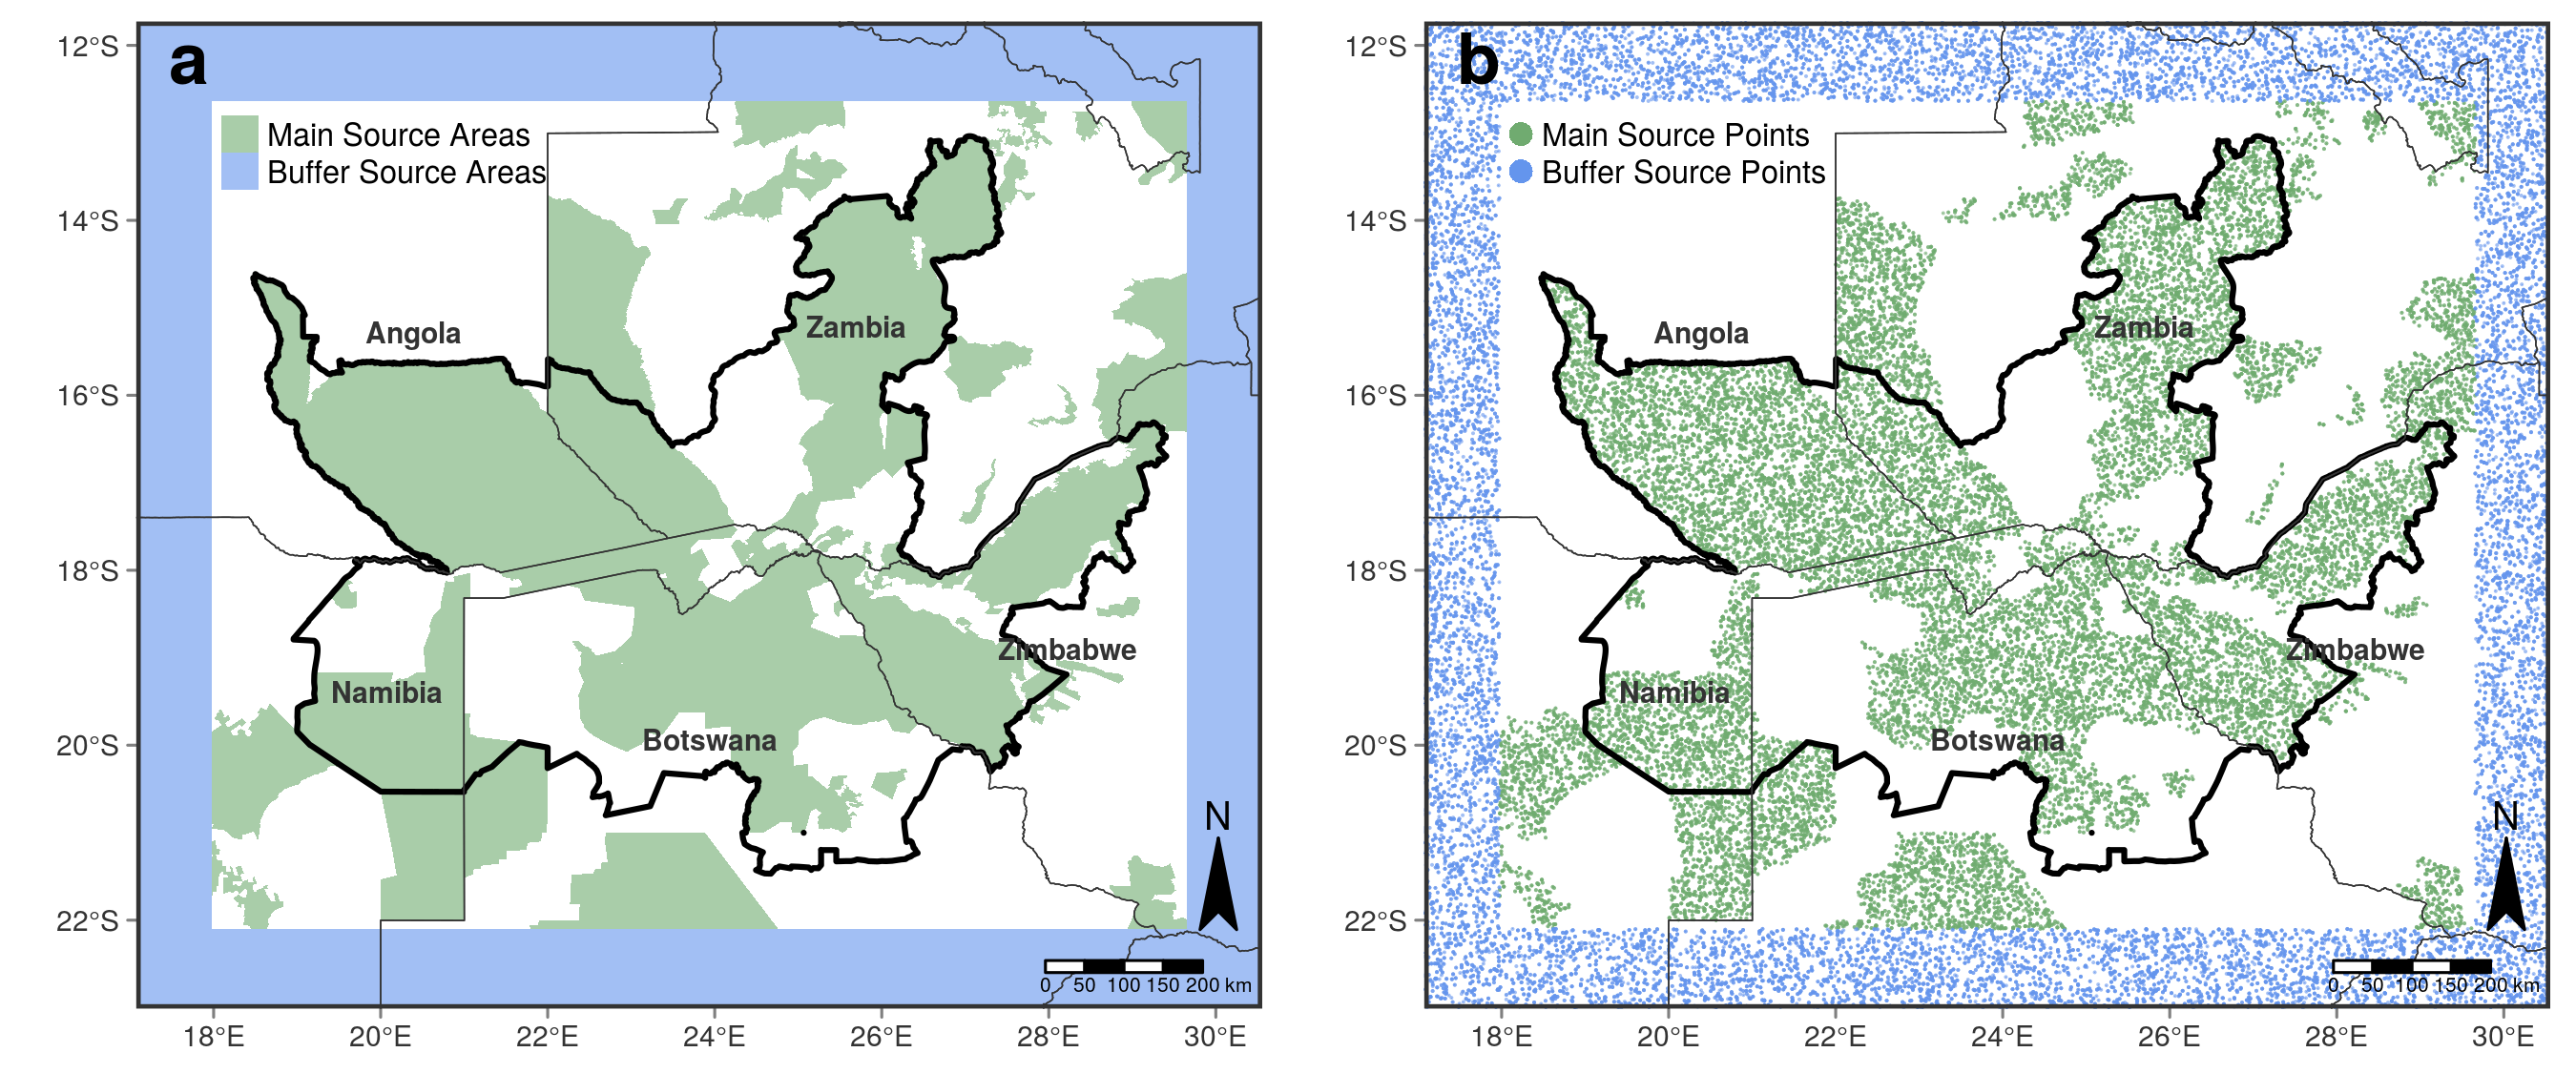
\includegraphics[width = \textwidth]{99_SourceAreas.png}
  \caption{(a) Different source areas from which we released virtual
   dispersers. We only considered contiguous protected areas (national parks,
   game reserves, and forest reserves) that were larger than 700
   km\textsuperscript{2}. This size corresponds to the average home range
   requirement for viable wild dog populations \citep{Pomilia.2015}. To render
   potential immigrants into the study system, we also initiated dispersers
   within a buffer zone (blue) surrounding the main study area. (b) Source
   points from which dipsersers were released. 50'000 dispersers were released
   within the main study area (green dots) and another 30'000 dispersers within
   the virtual buffer (blue dots).}
  \label{SourcePoints}
 \end{center}
\end{figure}

%------------------------------------------------------------------------------
%	Appendix S4: All Movement Models
%------------------------------------------------------------------------------
\newpage
\begin{landscape}
 \thispagestyle{empty}
 \section{Model Selection Results}
 % latex table generated in R 3.6.3 by xtable 1.8-4 package
 % Thu Jul  9 09:17:26 2020
 \begin{table}[hbpt]
  \caption{Results from the forward model selection procedure based on Akaike's
  Information Criterion (AIC; \citealp{Burnham.2002}). The model in the top row
  was the model that we used to simulate movement of dispersers. The base model
  upon which we based our movement model is depicted in the last row and was
  originally presented in \cite{Hofmann.2021}. We omitted all models with an AIC
  weight of zero from the table.}
  \label{ModelAICs}
  \begin{center}
   \resizebox{1.75\textwidth}{!}{
    \begin{threeparttable}
     \begin{tabular}{lllll}
      \toprule
      Covariates                                                                                                                           & AIC      & \(\Delta\)AIC & Weight & LogLik    \\
      \midrule
      \textbf{Base Model} + sl:LA + WA:sl + log(sl):cos(ta) + DTW:cos(ta) + WO:sl + HI:cos(ta) + SH:sl + DTW:sl + sl:cos(ta)               & 89392.88 & 0.00          & 0.15   & -44670.44 \\
      \textbf{Base Model} + sl:LA + WA:sl + log(sl):cos(ta) + DTW:cos(ta) + WO:sl + HI:cos(ta) + SH:sl + DTW:sl + sl:cos(ta) + SH:log(sl)  & 89393.92 & 1.04          & 0.09   & -44669.96 \\
      \textbf{Base Model} + sl:LA + WA:sl + log(sl):cos(ta) + DTW:cos(ta) + WO:sl + HI:cos(ta) + SH:sl + DTW:sl + sl:cos(ta) + DTW:log(sl) & 89394.13 & 1.25          & 0.08   & -44670.06 \\
      \textbf{Base Model} + sl:LA + WA:sl + log(sl):cos(ta) + DTW:cos(ta) + WO:sl + HI:cos(ta) + SH:sl + DTW:sl + sl:cos(ta) + WO:log(sl)  & 89394.25 & 1.37          & 0.08   & -44670.13 \\
      \textbf{Base Model} + sl:LA + WA:sl + log(sl):cos(ta) + DTW:cos(ta) + WO:sl + HI:cos(ta) + SH:sl + DTW:sl                            & 89394.36 & 1.48          & 0.07   & -44672.18 \\
      \textbf{Base Model} + sl:LA + WA:sl + log(sl):cos(ta) + DTW:cos(ta) + WO:sl + HI:cos(ta) + SH:sl + DTW:sl + sl:cos(ta) + log(sl):LA  & 89394.44 & 1.56          & 0.07   & -44670.22 \\
      \textbf{Base Model} + sl:LA + WA:sl + log(sl):cos(ta) + DTW:cos(ta) + WO:sl + HI:cos(ta) + SH:sl + DTW:sl + sl:cos(ta) + HI:sl       & 89394.56 & 1.68          & 0.07   & -44670.28 \\
      \textbf{Base Model} + sl:LA + WA:sl + log(sl):cos(ta) + DTW:cos(ta) + WO:sl + HI:cos(ta) + SH:sl + DTW:sl + sl:cos(ta) + WA:log(sl)  & 89394.57 & 1.69          & 0.07   & -44670.29 \\
      \textbf{Base Model} + sl:LA + WA:sl + log(sl):cos(ta) + DTW:cos(ta) + WO:sl + HI:cos(ta) + SH:sl + DTW:sl + sl:cos(ta) + WO:cos(ta)  & 89394.59 & 1.71          & 0.07   & -44670.30 \\
      \textbf{Base Model} + sl:LA + WA:sl + log(sl):cos(ta) + DTW:cos(ta) + WO:sl + HI:cos(ta) + SH:sl + DTW:sl + sl:cos(ta) + WA:cos(ta)  & 89394.63 & 1.75          & 0.06   & -44670.31 \\
      \textbf{Base Model} + sl:LA + WA:sl + log(sl):cos(ta) + DTW:cos(ta) + WO:sl + HI:cos(ta) + SH:sl + sl:cos(ta)                        & 89394.68 & 1.80          & 0.06   & -44672.34 \\
      \textbf{Base Model} + sl:LA + WA:sl + log(sl):cos(ta) + DTW:cos(ta) + WO:sl + HI:cos(ta) + SH:sl + DTW:sl + sl:cos(ta) + HI:log(sl)  & 89394.69 & 1.81          & 0.06   & -44670.35 \\
      \textbf{Base Model} + sl:LA + WA:sl + log(sl):cos(ta) + DTW:cos(ta) + WO:sl + HI:cos(ta) + SH:sl + DTW:sl + sl:cos(ta) + SH:cos(ta)  & 89394.84 & 1.96          & 0.06   & -44670.42 \\
      \hdashline
      \\
      \vdots                                                                                                                               & \vdots   & \vdots        & \vdots & \vdots    \\
      \\
      \hdashline
      \\
      \textbf{Base Model}: cos(ta) + sl + log(sl) + WA + WO + DTW + HI + SH                                                                & 90091.40 & 787.67        & 0.00   & -45030.70 \\
      \\
      \bottomrule
     \end{tabular}
     \begin{tablenotes}
      \item \textit{Note:} ta = Turning Angle, sl = Step Length, LA = Low Activity, WA = Water,
      DTW = Distance To Water, SH = Shrubs/Grassland, WO = Woodland, HI =
      Human Influence.
     \end{tablenotes}
    \end{threeparttable}
   }
  \end{center}
 \end{table}
 \vfill
 \raisebox{-1cm}{\makebox[\linewidth]{\thepage}}
\end{landscape}


%------------------------------------------------------------------------------
%	Appendix S5: Most Parsimonious Movement Models
%------------------------------------------------------------------------------
\newpage
\section{Movement Model}
\begin{table}[htbp]
 \begin{center}
  \caption{Most parsimonious movement model for dispersing wild dogs. The model
   consists of a movement kernel, a habitat kernel, and their interactions. The
   movement kernel describes preferences with regards to movement behavior,
   whereas the habitat kernel describes preferences with respect to habitat
   conditions. Interactions between the two kernels indicate that movement
   preferences are contingent on habitat conditions. Note that all covariates
   were standardized to a mean of zero and standard deviation of 1. Plots to aid
   with the interpretation of this model are given in Appendix S2.}
  \label{MovementModelNumbers}
  \resizebox{\textwidth}{!} {
   \begin{threeparttable}
    \begin{tabular}{llrrrc}
     \toprule
     Kernel & Covariate                                       & Coefficient & SE    & p-value     & Sign. \\
     \midrule
     \multirow{5}{*}{Habitat Kernel}
            & Water                                           & -0.546      & 0.112 & \(<\) 0.001 & ***   \\
            & DistanceToWater \textsuperscript{0.5}           & -0.390      & 0.231 & 0.092       & *     \\
            & Woodland                                        & -0.364      & 0.086 & \(<\) 0.001 & ***   \\
            & Shrubs/Grassland                                & 0.288       & 0.092 & 0.002       & ***   \\
            & HumanInfluence                                  & -0.535      & 0.229 & 0.019       & **    \\
     \hdashline
     \multirow{6}{*}{Movement Kernel}
            & sl                                              & 0.075       & 0.037 & 0.042       & **    \\
            & cos(ta)                                         & 0.105       & 0.031 & 0.001       & ***   \\
            & log(sl)                                         & 0.146       & 0.051 & 0.004       & ***   \\
            & cos(ta) : sl                                    & 0.049       & 0.026 & 0.064       & *     \\
            & cos(ta) : log(sl)                               & 0.076       & 0.026 & 0.003       & ***   \\
            & sl : LowActivity                                & -0.917      & 0.113 & \(<\) 0.001 & ***   \\
     \hdashline
     \multirow{5}{*}{Interactions}
            & sl : Water                                      & -0.305      & 0.076 & \(<\) 0.001 & ***   \\
            & sl : Woodland                                   & -0.089      & 0.039 & 0.023       & **    \\
            & sl : Shrubs/Grassland                           & 0.124       & 0.058 & 0.032       & **    \\
            & sl : DistanceToWater \textsuperscript{0.5}      & -0.058      & 0.031 & 0.056       & *     \\
            & cos(ta) : HumanInfluence                        & -0.040      & 0.022 & 0.070       & *     \\
            & cos(ta) : DistanceToWater \textsuperscript{0.5} & 0.063       & 0.026 & 0.017       & **    \\
     \bottomrule
    \end{tabular}
    \begin{tablenotes}
     \item \textit{Significance codes: * \(p < 0.10\) \quad ** \(p < 0.05\)
      \quad *** \(p < 0.01\)}
    \end{tablenotes}
   \end{threeparttable}
  }
 \end{center}
\end{table}


%------------------------------------------------------------------------------
%	Appendix S6: Movement Model interpretation
%------------------------------------------------------------------------------
\newpage
% \newgeometry{left=35mm,right=35mm,top=25mm,bottom=5mm,footskip=0pt}
\section{Movement Model Interpretation}
To ease with the interpretation of the most parsimonious movement model, we
followed recommendations published in \cite{Fieberg.2021} and produced a series
of plots highlighting how the habitat and movement kernel depended on covariate
values (\Cref{Interpretation}). To visualize the movement kernel and its
interactions with other covariates, we used model estimates and updated our
tentative distribution parameters for turning angles (von Mises distribution
with concentration \(\kappa = 0\)) and step lengths (gamma distribution with
scale \(\theta\) = 6'308 and shape \(k\) = 0.37) by applying the function
\textsf{update\_vonmises()} from the R-package \textsf{amt} \citep{Amt.2019}.
This allowed us to compute probability densities of turning angles and step
lengths under varying values of the associated covariates, while holding all
other covariates constant (\Cref{Interpretation}, a1-a8). Moreover, we
investigated the habitat kernel by computing relative selection strengths (RSS)
between a set of steps where values of the covariate of interest was varied to a
reference step where the covariate value was fixed to its centered value. To
illustrate model uncertainty, we also generated large-sample confidence
intervals using standard errors associated with each model estimate
(\Cref{Interpretation}, b1-b5).

\begin{figure}[hbtp]
 \begin{center}
  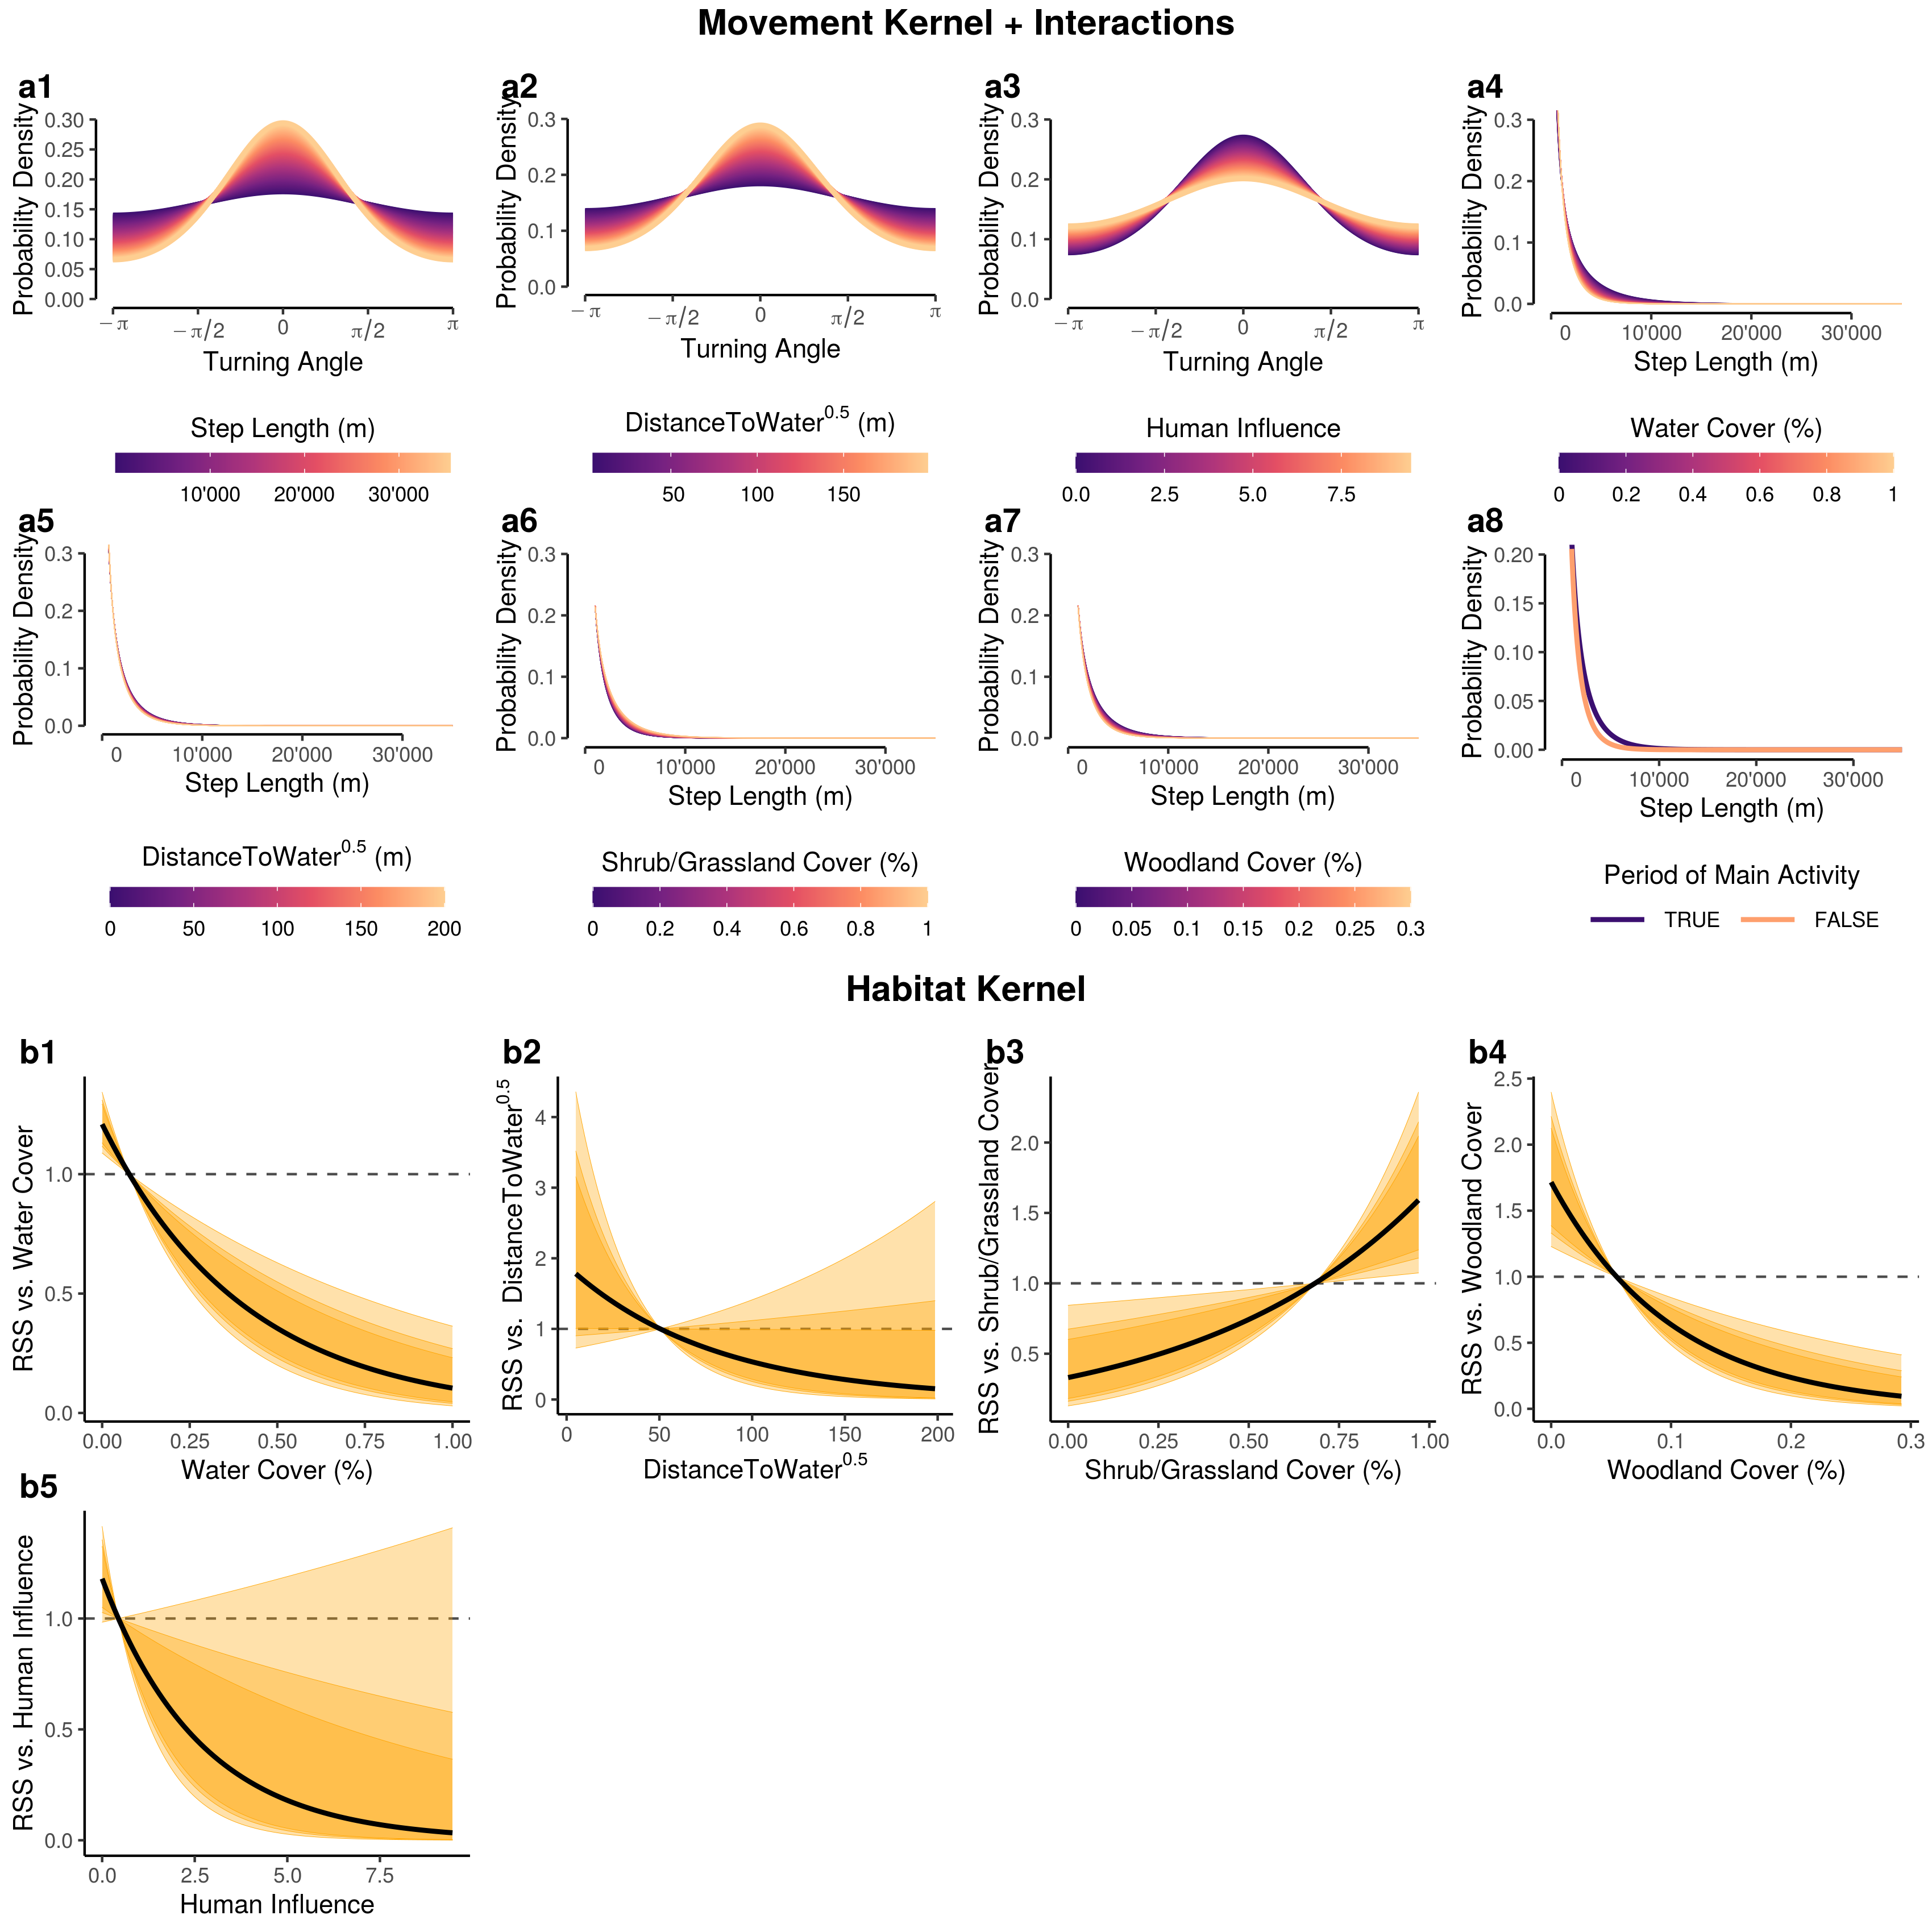
\includegraphics[width = \textwidth]{99_MovementModelInterpretation.png}
  \caption{Auxiliary plots that help with the interpretation of the most
  parsimonious movement model from Table S1. The plots were generated following
  recommendations reported in \cite{Fieberg.2021}. Subplots a1 to a8 highlight
  dispersing wild dogs' movement kernel and indicate how the kernel is
  influenced by interactions with other covariates. Subplots b1 to b5 depict
  results from dispersing wild dogs' habitat kernel and highlight differences in
  predicted relative selection scores (RSS) when varying values of the covariate
  of interest. For each covariate, predictions were made on the range of values
  that was observed in the real data, assuming that all other covariates were
  centered and that steps were realized during periods of ``high'' wild dog
  activity. Plot a1, for example, can be interpreted as follows: the probability
  of realizing a step with a low turning angle is much higher when the
  corresponding step is large. Moreover, b1 can be interpreted as follows:
  relative probability of using a step decreases as the amount of water cover
  along the step increases.}
  \label{Interpretation}
 \end{center}
\end{figure}
% \restoregeometry

%------------------------------------------------------------------------------
%	Appendix S7: Convergence
%------------------------------------------------------------------------------
\newpage
\section{Convergence}
\begin{figure}[htbp]
  \begin{center}
    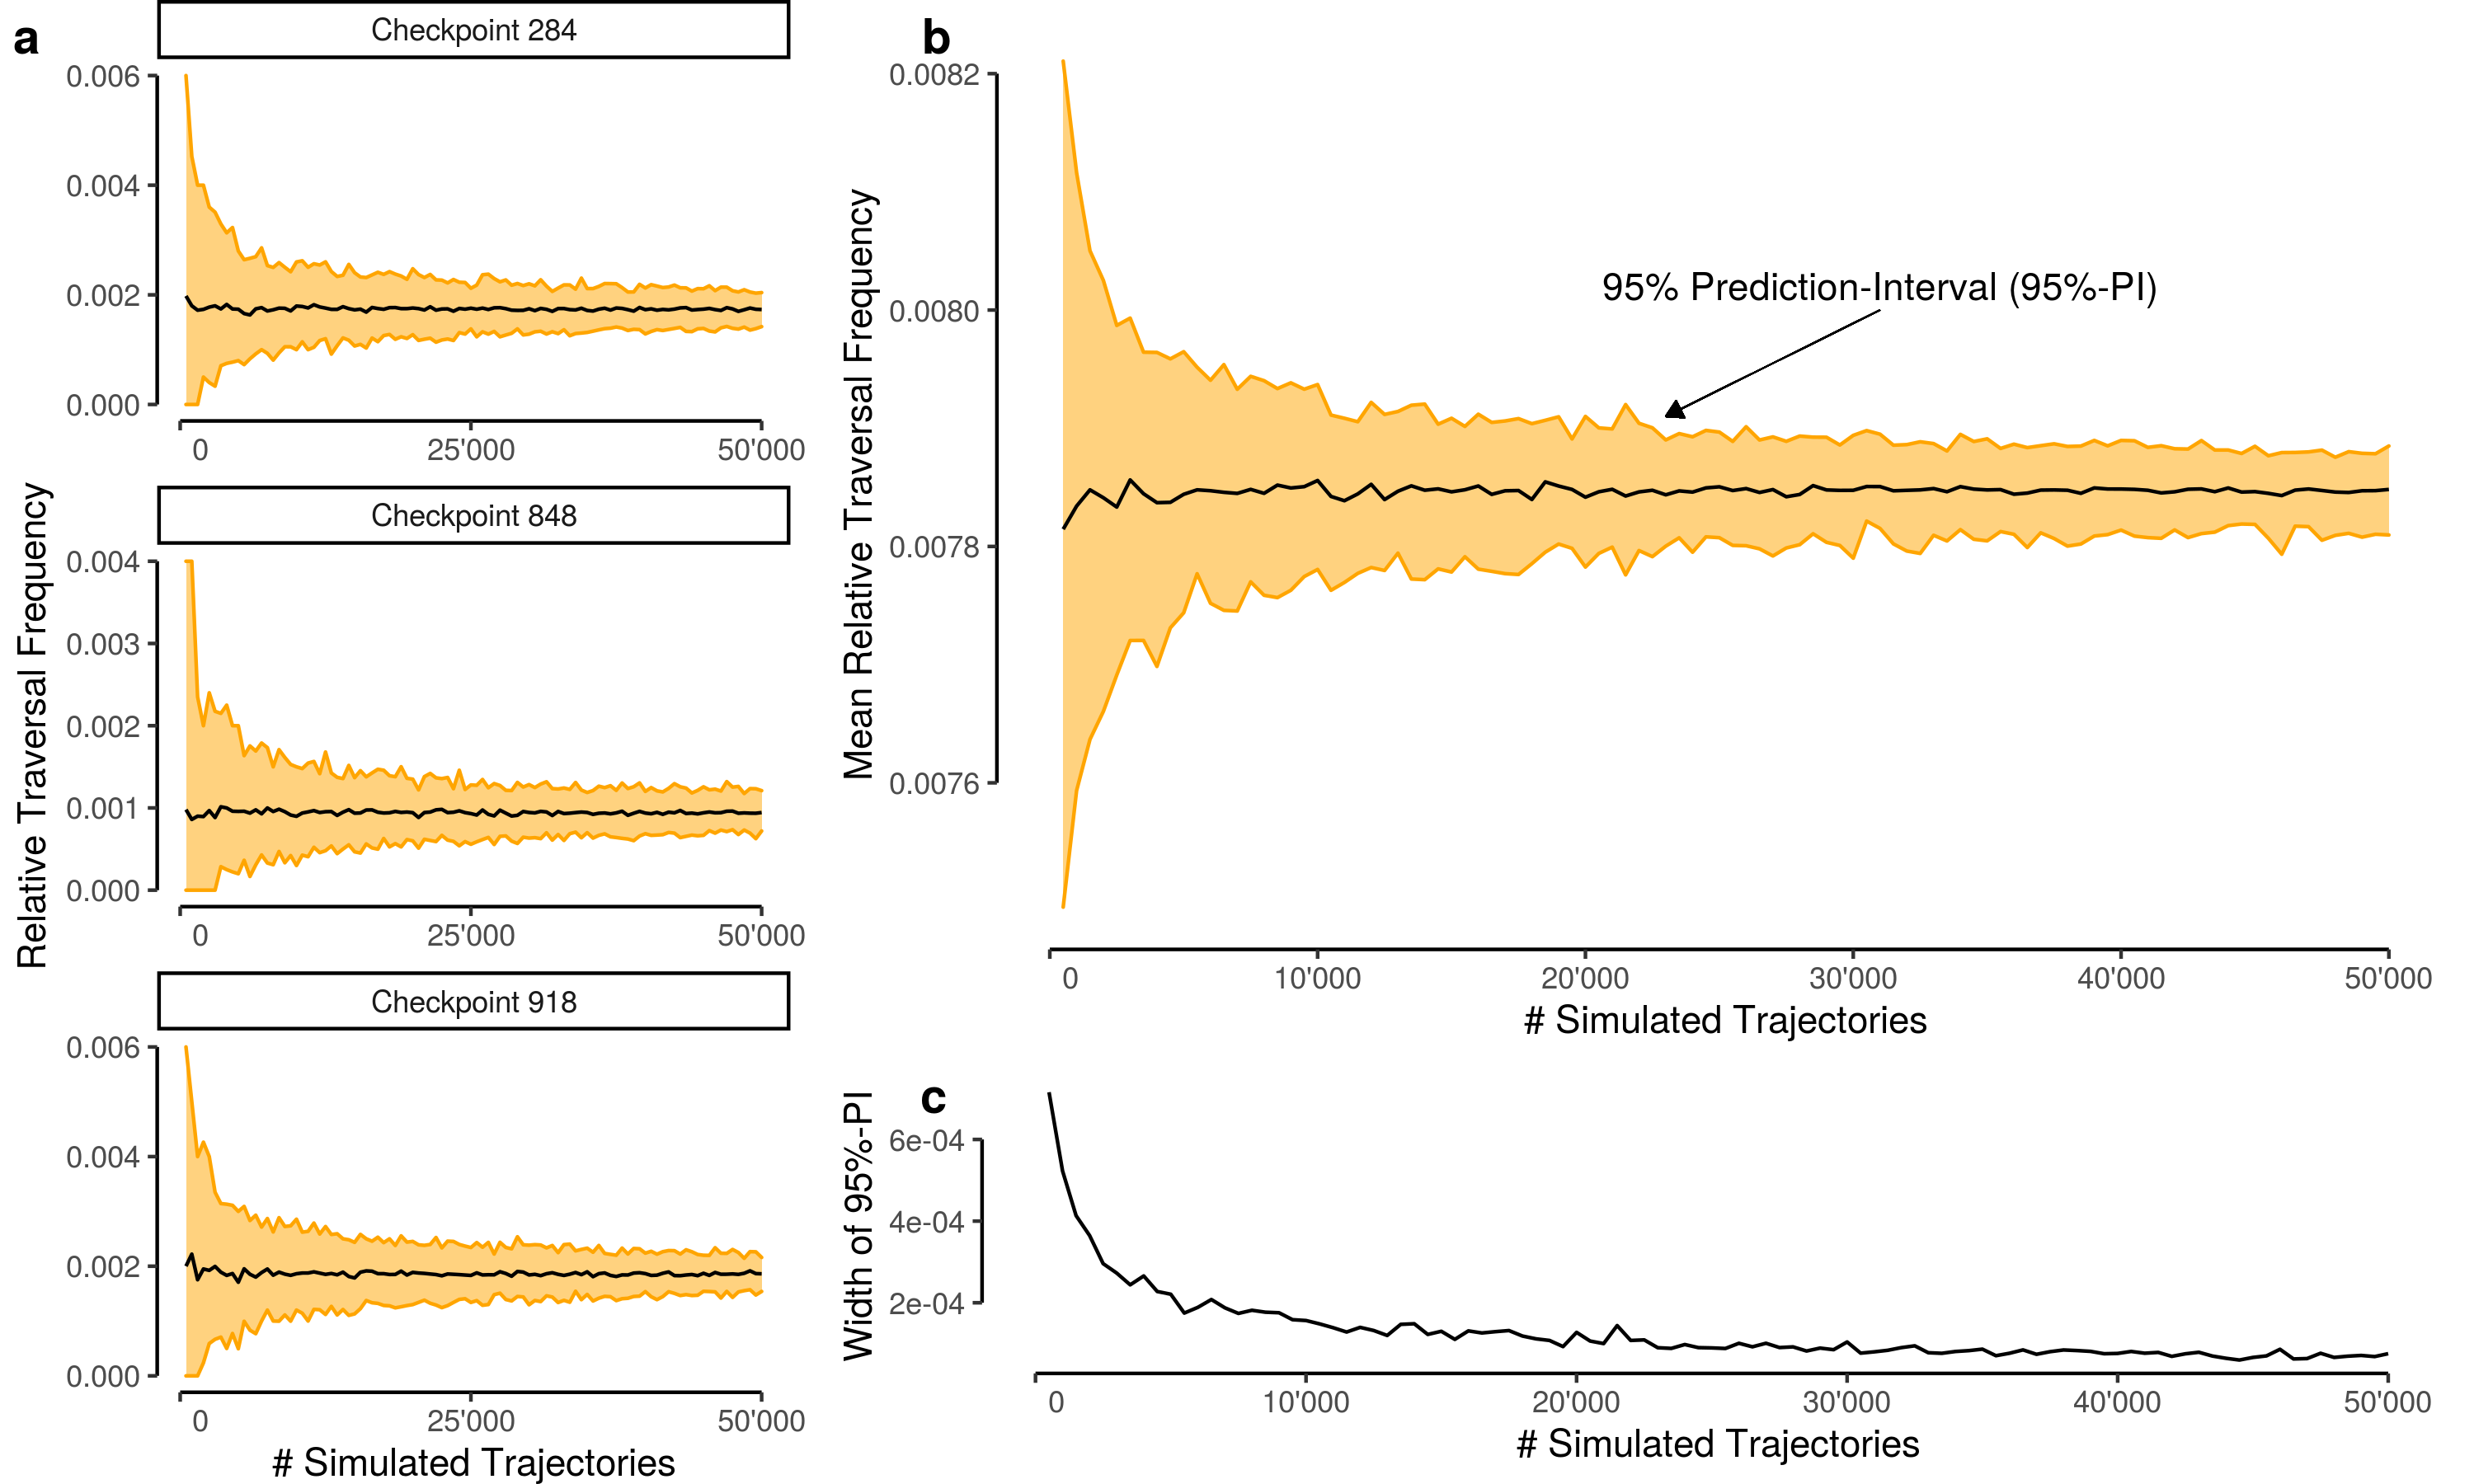
\includegraphics[width=\textwidth]{99_Convergence}
    \caption{Relative traversal frequency through 1'000 checkpoints (5 km x 5
    km) distributed randomly across the study area. The relative traversal
    frequency is plotted against the number of simulated individuals to
    visualize how quickly the metric converges to a steady state. (a) Replicated
    (100 times) relative traversal frequencies across three randomly chosen
    checkpoints as well as the corresponding 95\% prediction interval (PI). (b)
    Averaged relative traversal frequency across all checkpoints and replicates
    including a 95\% PI. (c) Width of the PI in relation to the number of
    simulated dispersers.}
    \label{Convergence}
  \end{center}
\end{figure}

%------------------------------------------------------------------------------
%	Appendix S8: Heatmaps
%------------------------------------------------------------------------------
\newpage
\newgeometry{left=35mm,right=35mm,top=25mm,bottom=5mm,footskip=0pt}
\section{Heatmaps in Relation to the Number of Simulated Steps}
\begin{figure}[hbtp]
 \begin{center}
  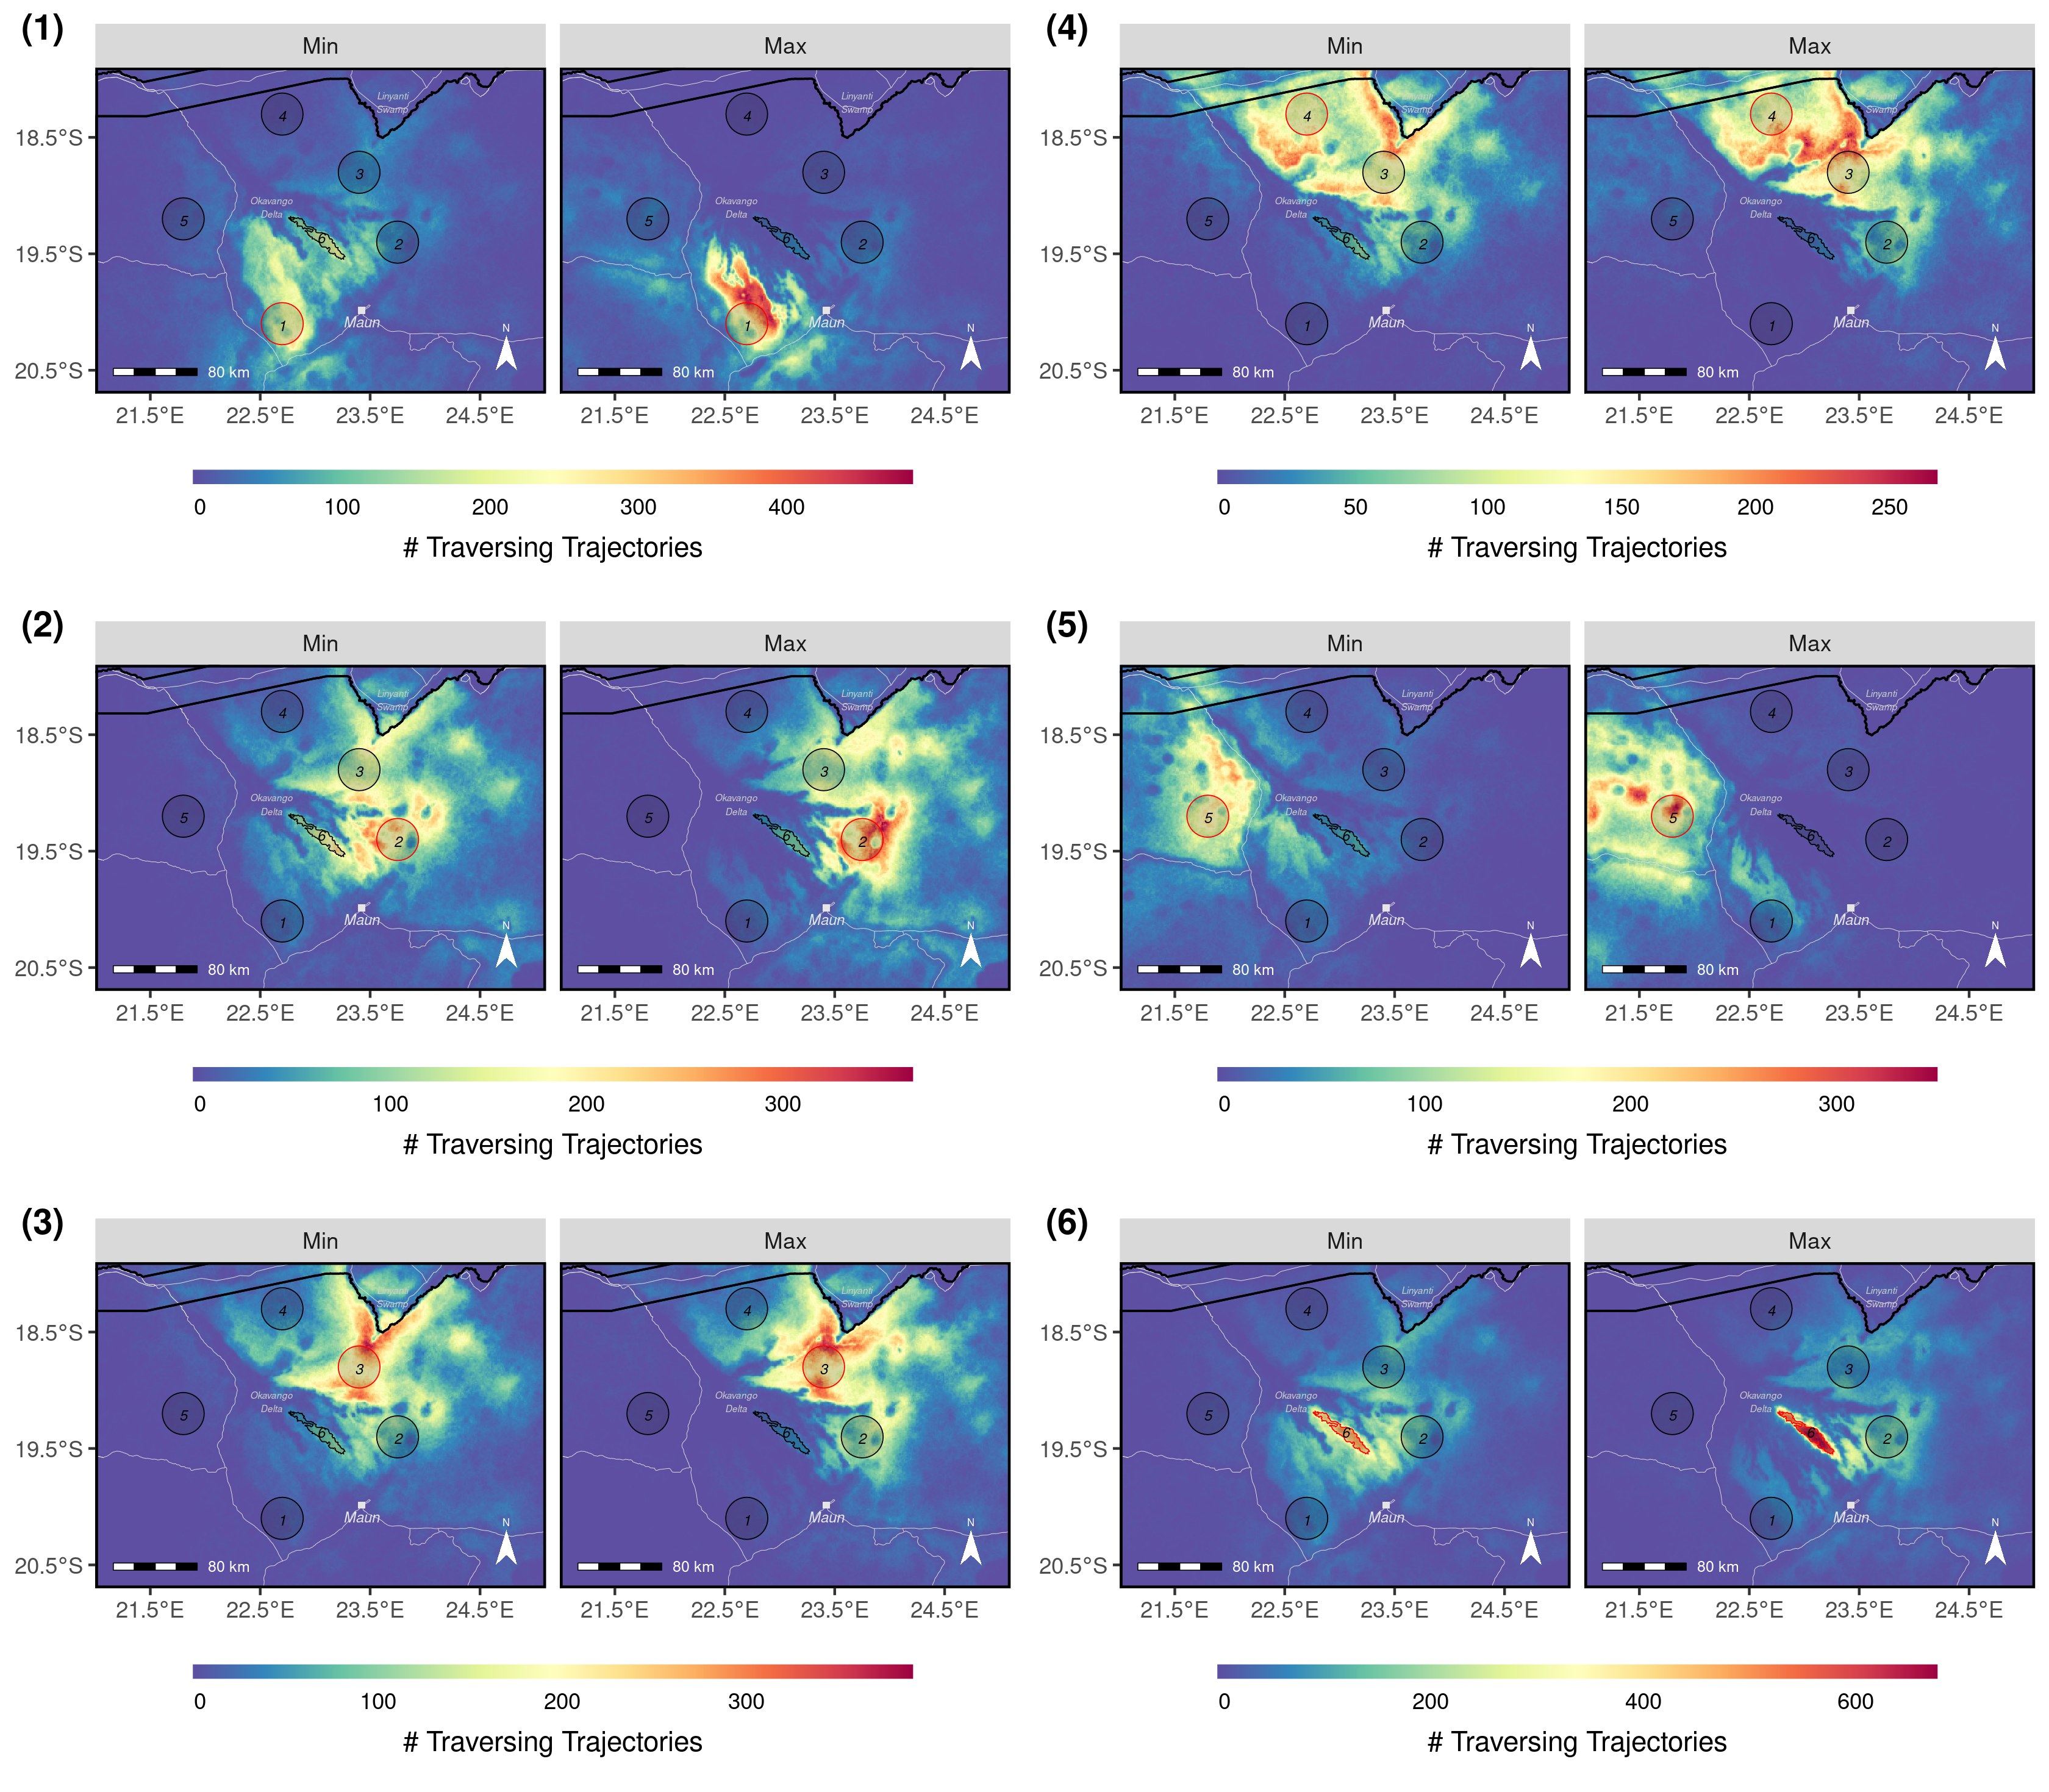
\includegraphics[width = 0.86\textwidth]{99_HeatmapsIndividual.png}
  \caption{Heatmaps produced when considering 125, 500, and 2000 simulated
   steps, respectively. The left panel (a1, a2, a3) was generated based on
   simulations initiated within the main study area, the right panel (b1, b2,
   b3) was generated based on simulations initiated within the buffer area. To
   produce the heatmap presented in the main manuscript (Figure 5), we tallied
   the values from maps a3 and b3.}
  \label{Heatman}
 \end{center}
\end{figure}
\restoregeometry

%------------------------------------------------------------------------------
%	Appendix S9: Evolution of Betweenness Maps
%------------------------------------------------------------------------------
\newpage
\newgeometry{left=35mm,right=35mm,top=25mm,bottom=10mm,footskip=0pt}
\section{Betweenness Maps in Relation to the Number of Simulated Steps}
\begin{figure}[hbtp]
 \begin{center}
  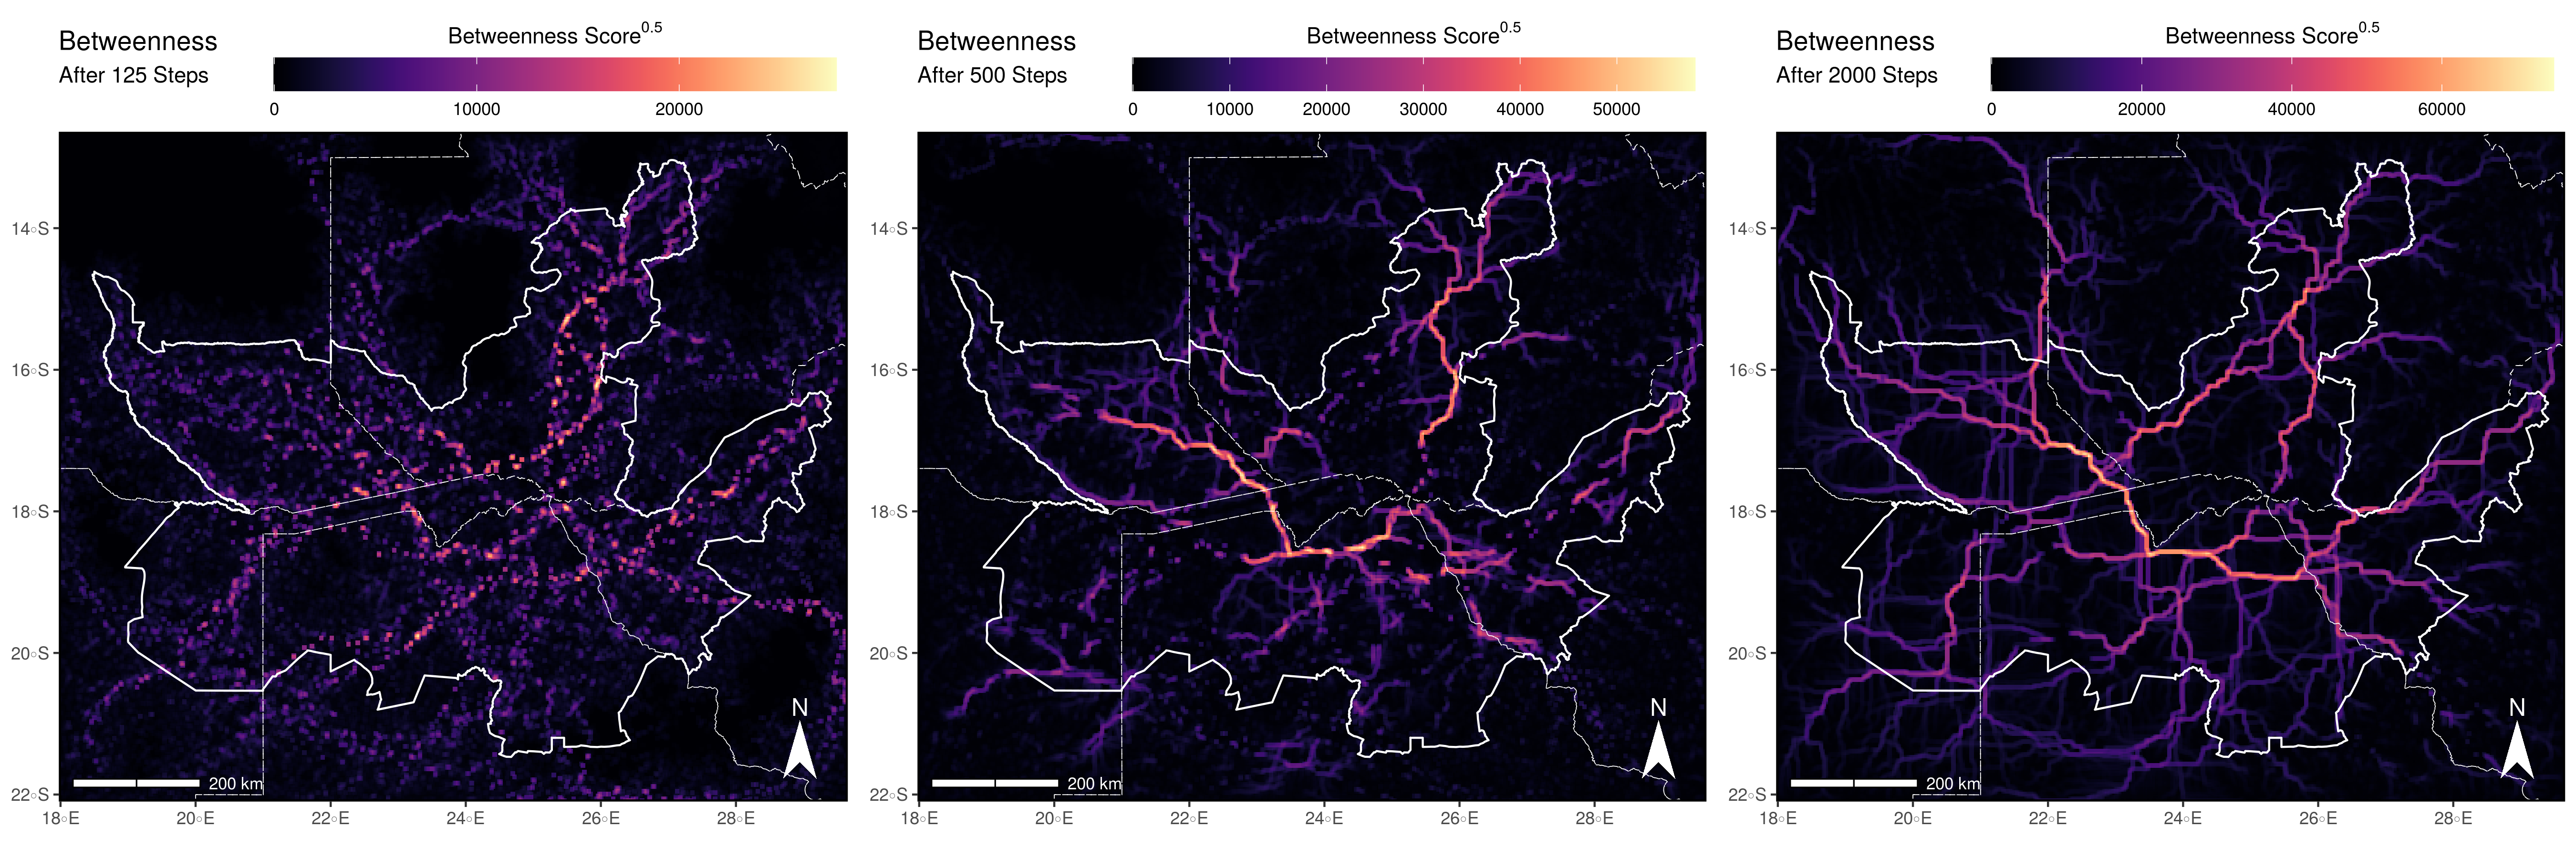
\includegraphics[width = 0.86\textwidth]{99_BetweennessIndividual.png}
  \caption{Maps of betweenness scores produced when considering (a) 125, (b)
   500, (c) and 2000 simulated steps, respectively. A high betweenness score
   indicates that the respective area has a high importance for linking other
   regions in the study area.}
  \label{Betweenness}
 \end{center}
\end{figure}
\restoregeometry

%------------------------------------------------------------------------------
%	Appendix S11: Map Comparison
%------------------------------------------------------------------------------
\newpage
\section{Comparison of Traversal Frequencies and Betweenness Scores Inside and Outside KAZA-TFCA}
\begin{figure}[hbtp]
 \begin{center}
  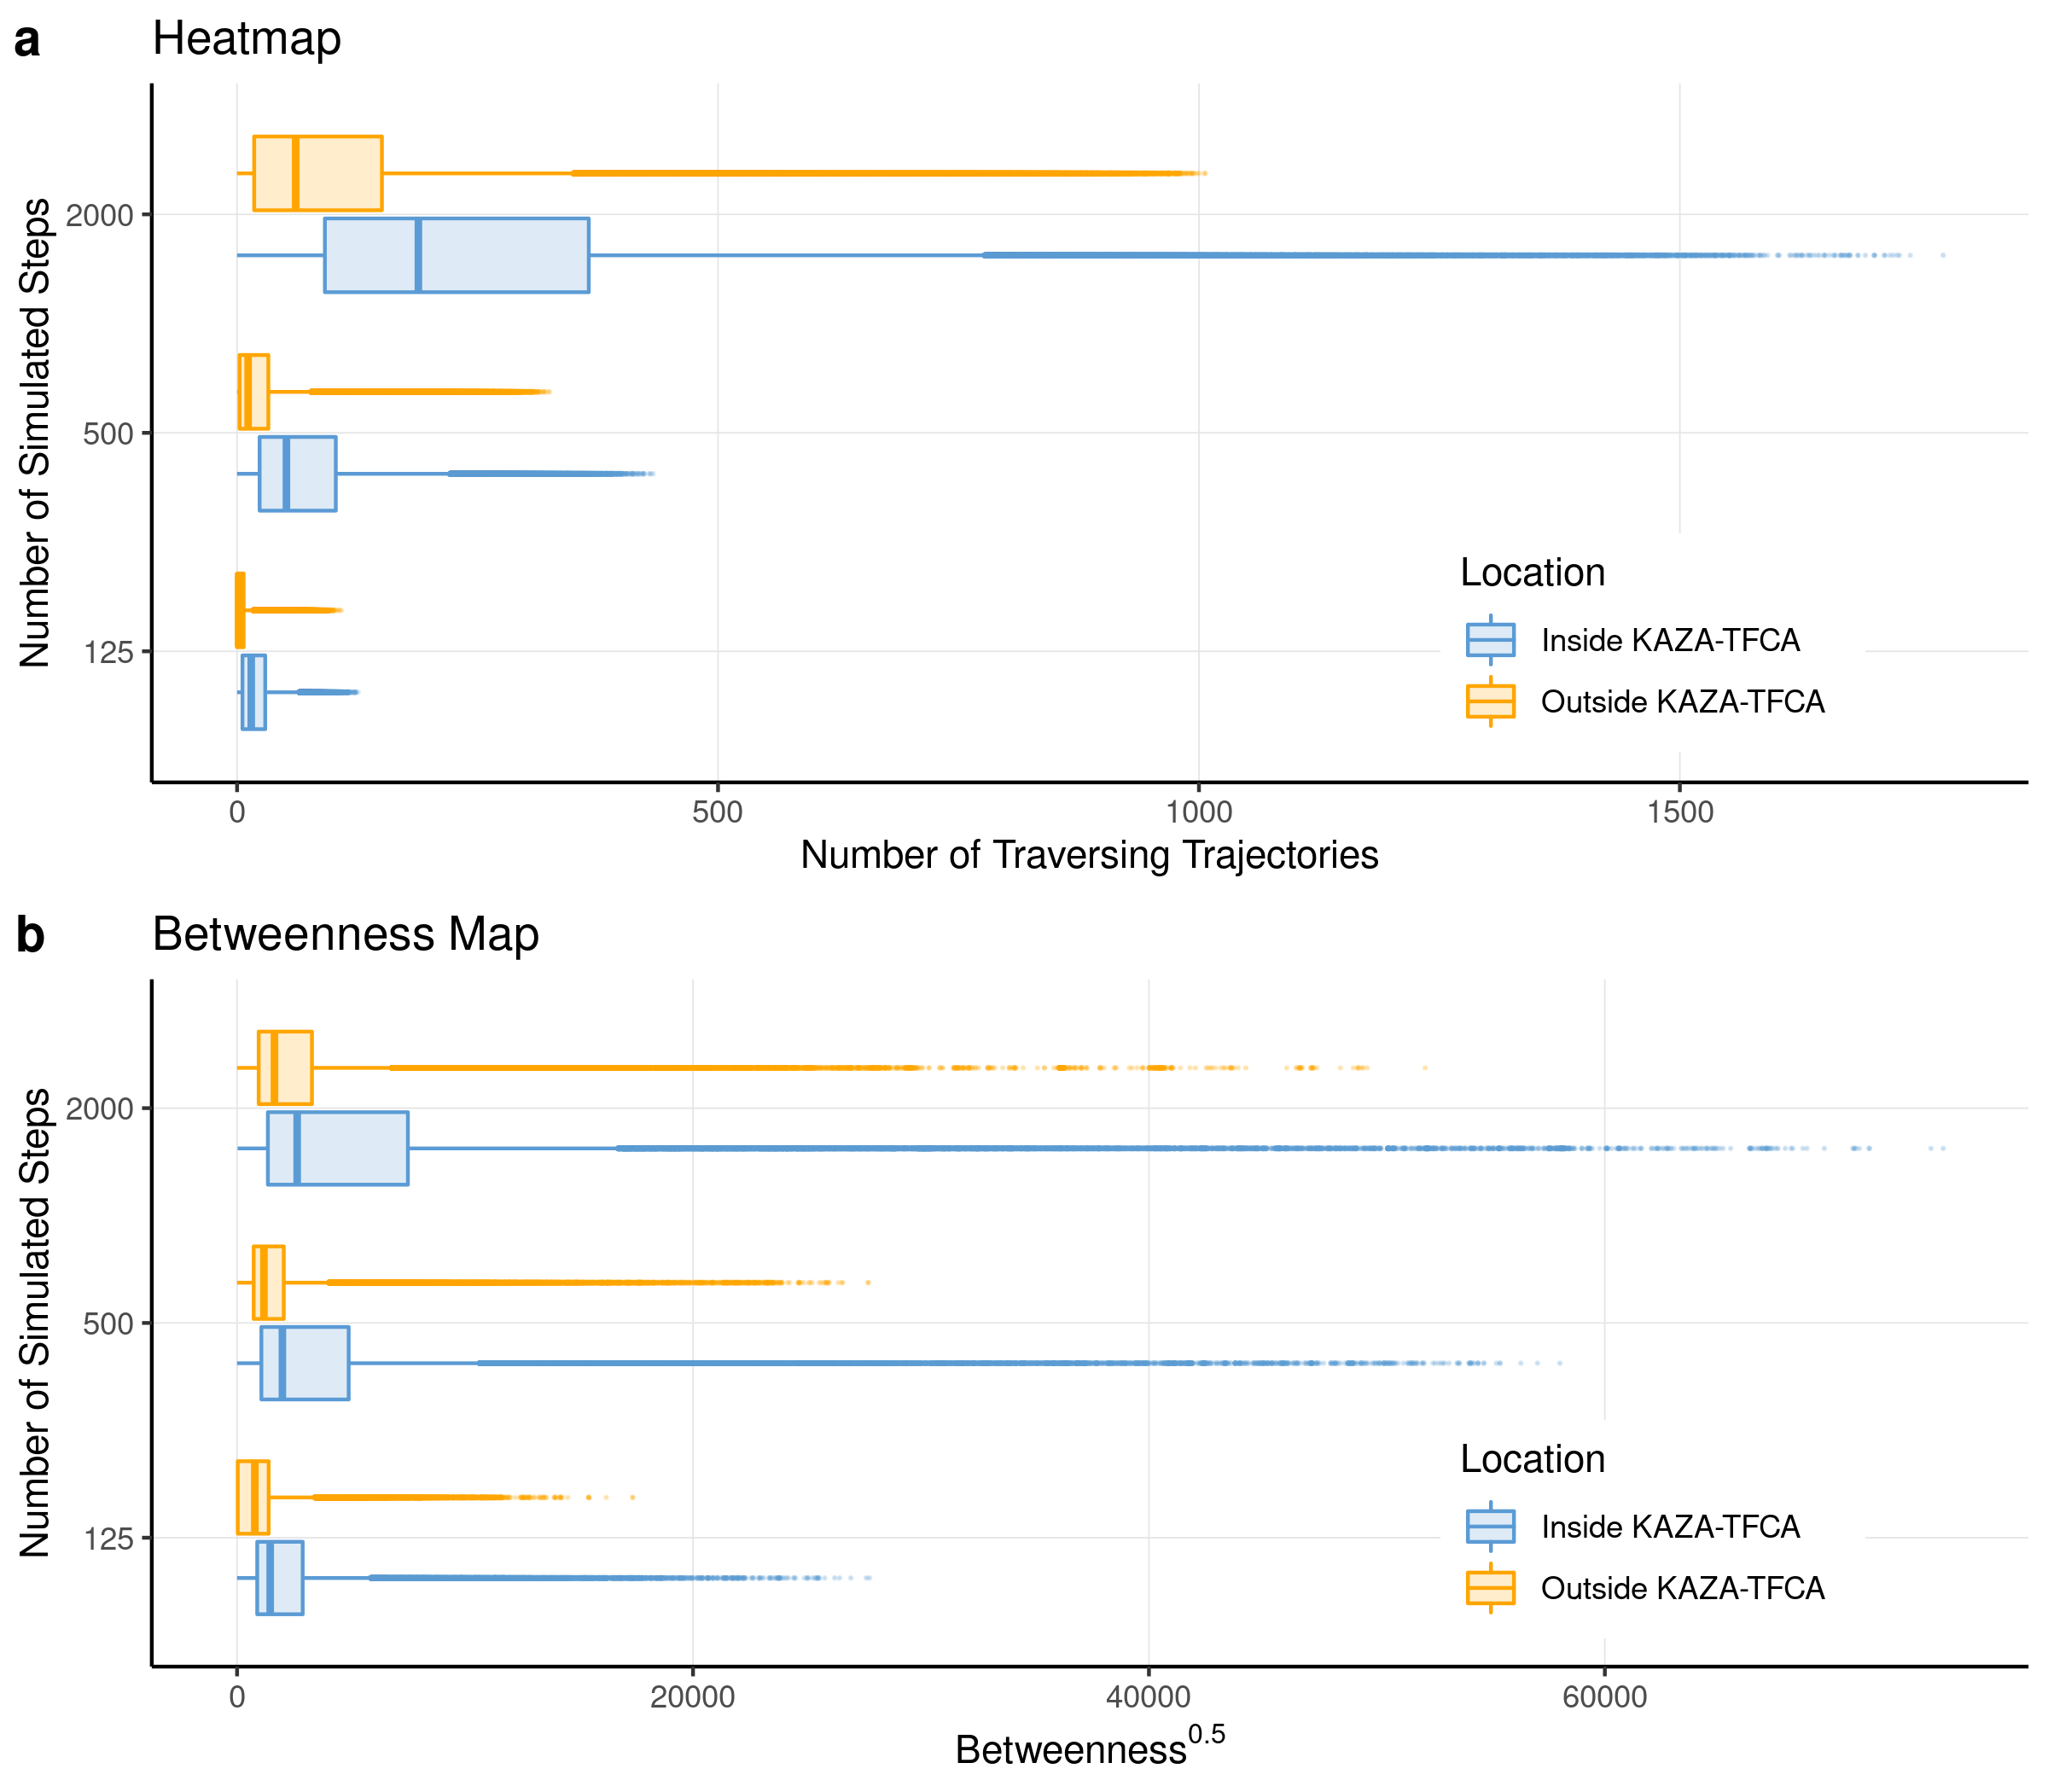
\includegraphics[width = \textwidth]{99_MapComparison.png}
  \caption{Comparison of values from the heatmap and betweenness map inside
  (blue) and outside (orange) the KAZA-TFCA borders.}
  \label{MapComparison}
 \end{center}
\end{figure}

\begin{figure}[hbtp]
 \begin{center}
  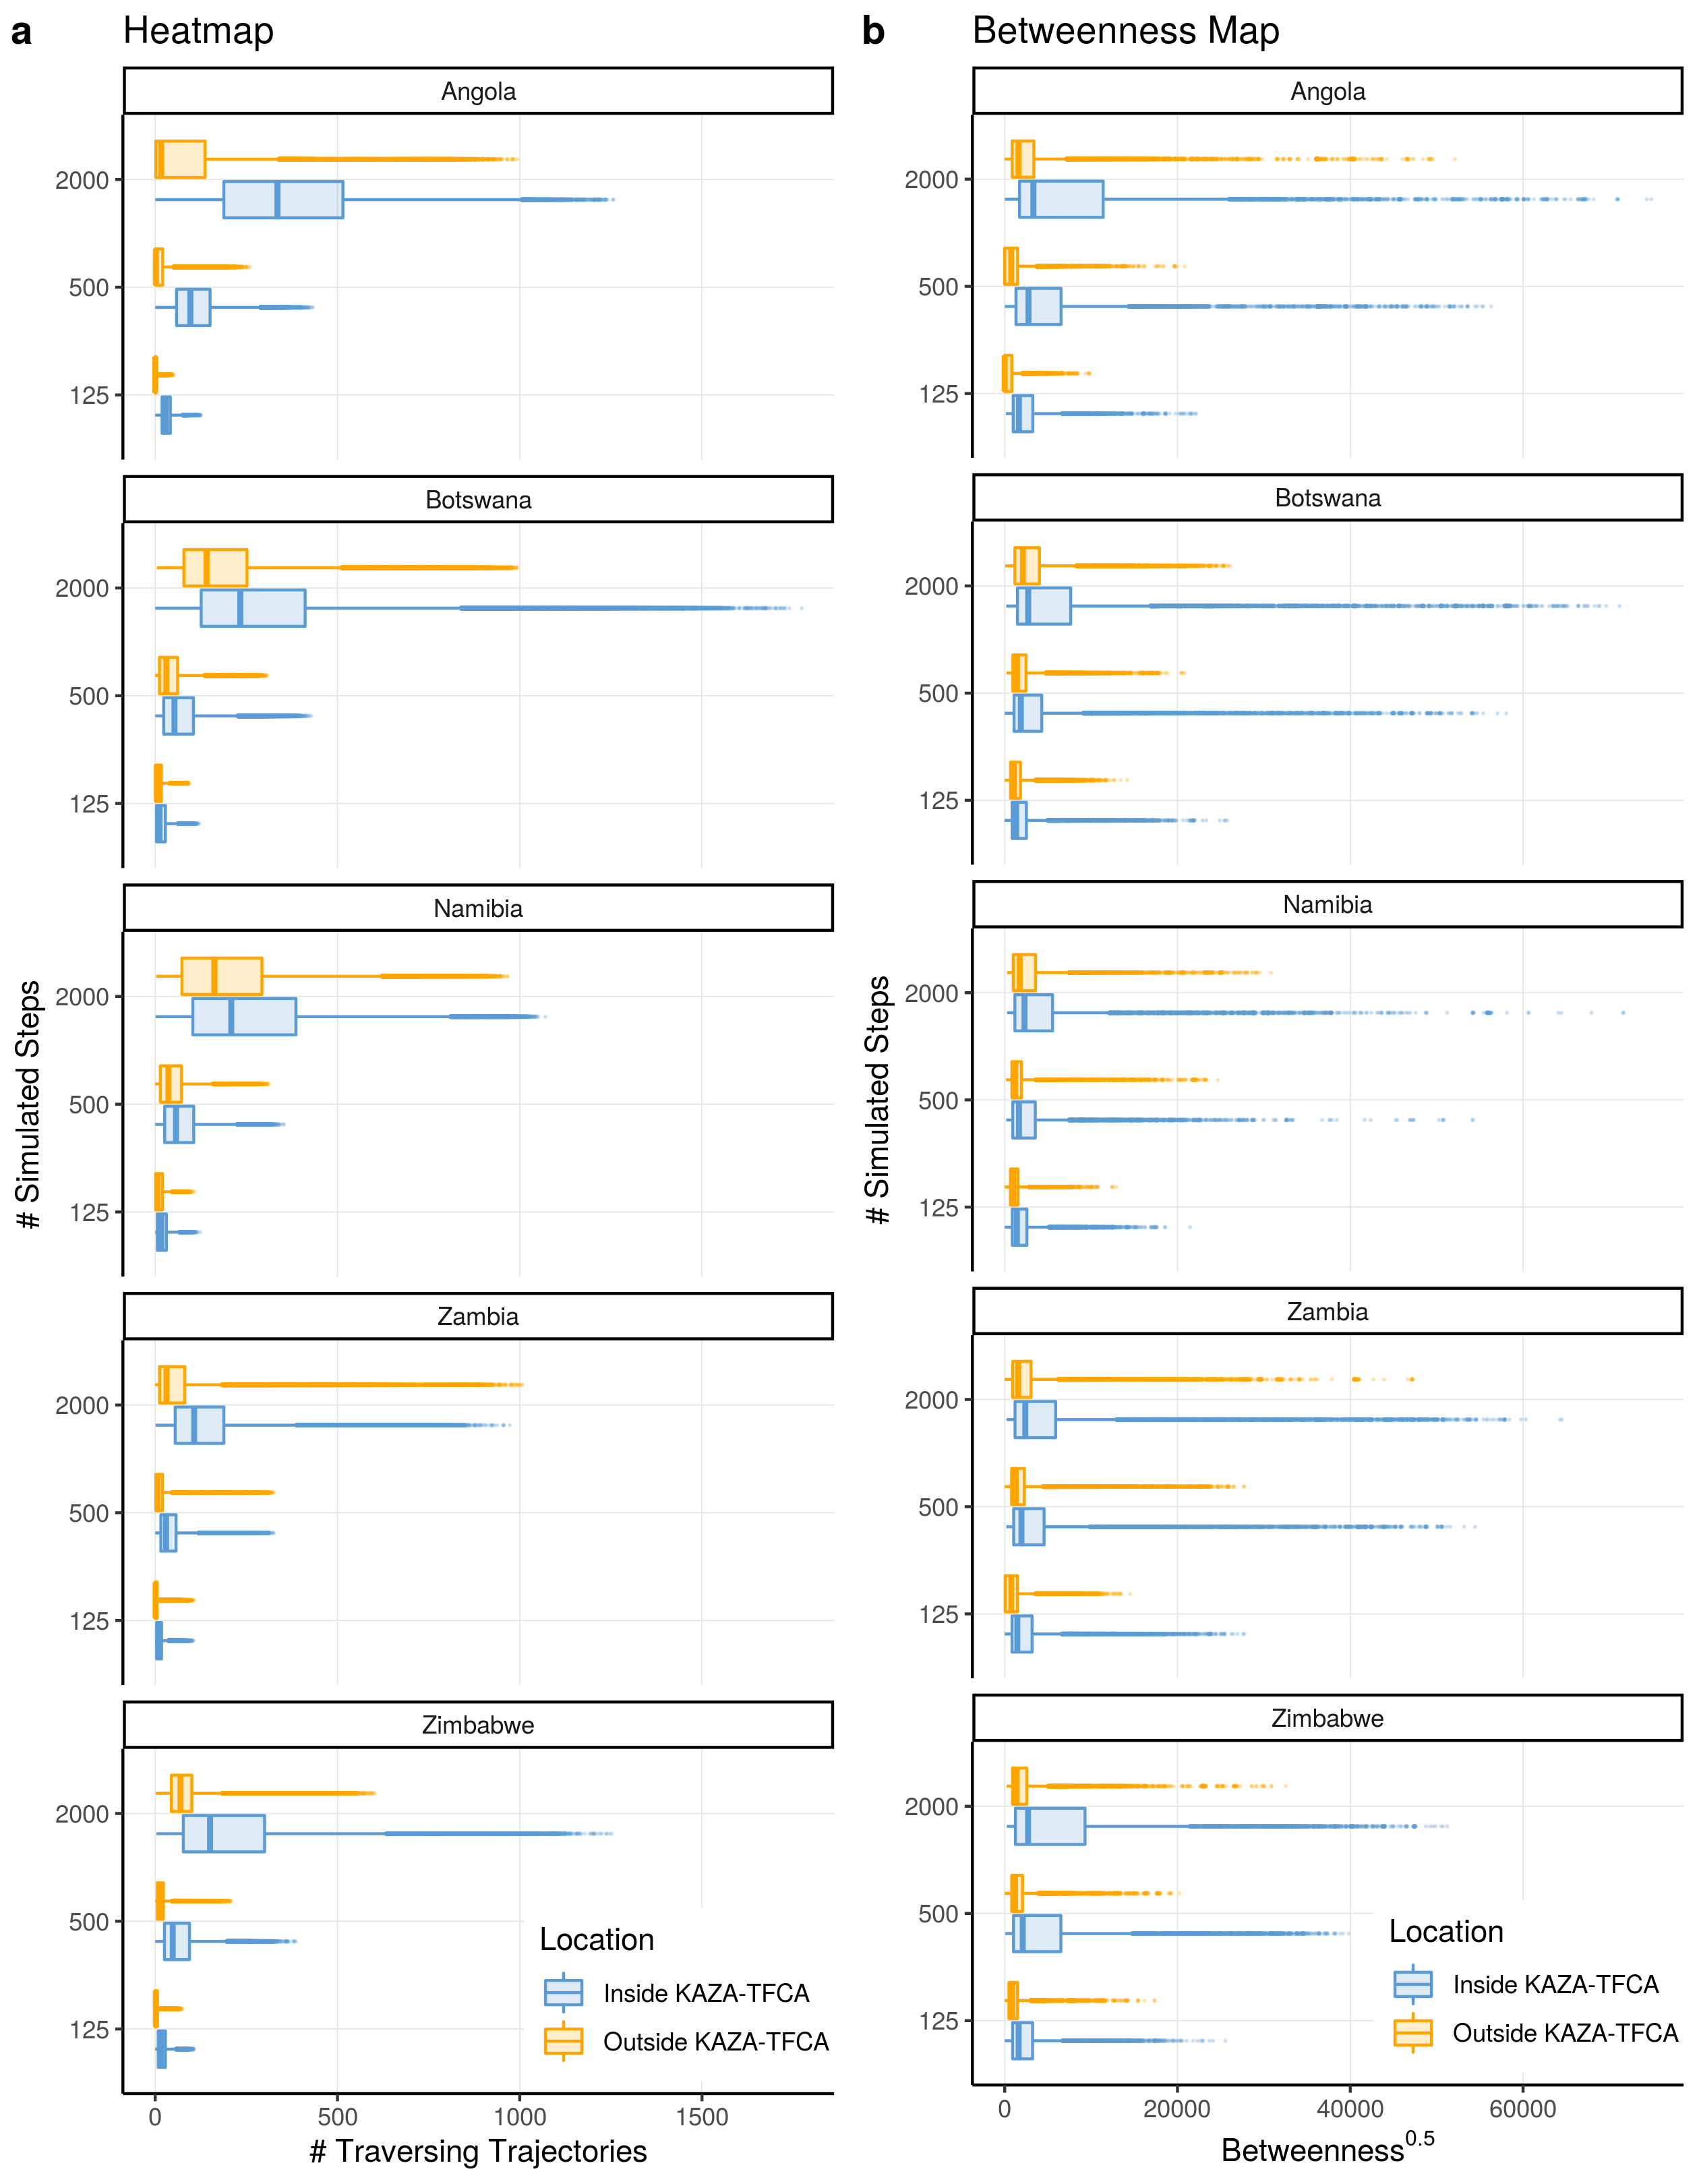
\includegraphics[width = \textwidth]{99_MapComparisonCountries.png}
  \caption{Comparison of values from the heatmap and betweenness map inside
  (blue) and outside (orange) the KAZA-TFCA borders within different countries.}
  \label{MapComparisonCountries}
 \end{center}
\end{figure}

%------------------------------------------------------------------------------
%	Appendix S12: Areas Reached
%------------------------------------------------------------------------------
\newpage
\section{Dispersal into other National Parks}
\begin{figure}[hbtp]
 \begin{center}
  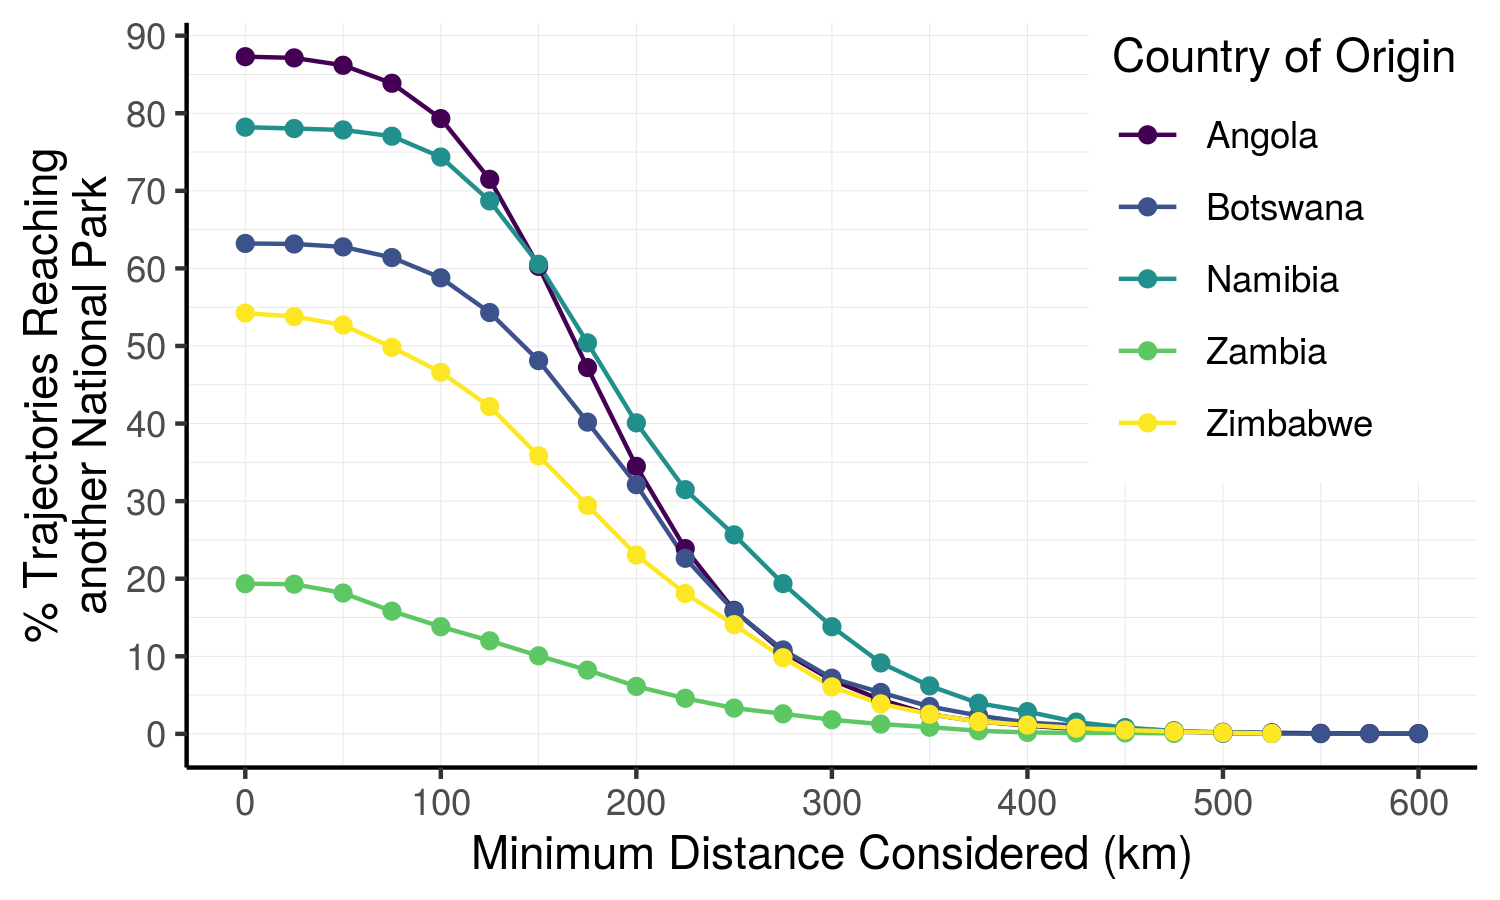
\includegraphics[width = \textwidth]{99_AreasReached.png}
  \caption{Relative number of simulated dispersal trajectories that successfully
  moved from one national park into another that is at least as far away as
  indicated on the x-axis. Percentages are given in relation to the number of
  simulated individuals from the national parks in the respective countries. For
  example, over 85\% of all individuals originating from a national park in
  Angola moved from their natal national park into another one. However, the
  percentage gradually decreases as only national parks at higher euclidean
  distances are considered.}
  \label{AreasReached}
 \end{center}
\end{figure}

\newpage
\begingroup
\singlespacing
\bibliography{Literatur}
\endgroup

\end{document}
